\subsection{Introduction}
\begin{frame}{}
    \LARGE VAE: \textbf{Introduction}
\end{frame}

\begin{frame}{From a Point to a Distribution}
\begin{itemize}
    \item An \textbf{autoencoder} learns a mapping: each input $x$ lands on \textbf{one point} $z$ in latent space. We just saw why sampling that space fails: nothing controls what lies \emph{between} the points.
    \item A \textbf{VAE} changes what the encoder outputs: instead of a point, it predicts the parameters of a \textbf{distribution}, a mean $\mu(x)$ and a standard deviation $\sigma(x)$, and $z$ is \textbf{sampled} from $\mathcal{N}(\mu(x), \sigma^2(x))$.
    \item Decoding from a sampled \textbf{region} rather than a fixed point forces nearby latents to decode to similar outputs: the space becomes smooth by construction.
    \item Everything that follows (reparameterization, the KL term, the ELBO) exists to make this simple idea trainable and useful.
\end{itemize}
\end{frame}


\begin{frame}[allowframebreaks]{Introduction}
  \begin{itemize}
    \item We want a \textbf{generative model}: given a latent $\mathbf{z}$ drawn from a prior, it outputs a new sample from the data distribution.
    \item To make the latent space $Z$ continuous, let's choose it to be Gaussian.
    \item So now, we want to estimate the true parameters $\theta^*$ of this generative model.
\end{itemize}
    \begin{figure}
        \centering
        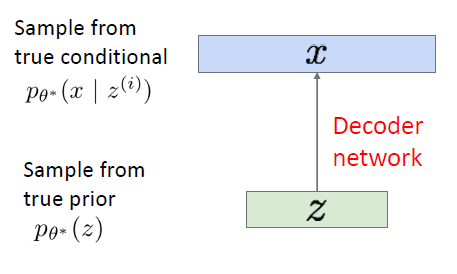
\includegraphics[height=0.45\textheight, width=\textwidth, keepaspectratio]{./images/vae/abstract_model.png}
        \caption*{\scriptsize Source: Stanford CS231n, Lecture 13 ``Generative Models'' (Fei-Fei Li, Justin Johnson, Serena Yeung), 2017.}
    \end{figure}

\framebreak

\begin{itemize}
  \item \textbf{Probabilistic Encoder:} Instead of encoding an input \( x \) to a fixed point \( z \), the encoder learns a distribution over the latent variable \( z \) conditioned on the input:
  \[ q(z \mid x) \]
  Typically, this is a multivariate Gaussian with parameters \( \mu(x) \) and \( \sigma(x) \) learned by a neural network.

  \framebreak
  
  \item \textbf{Probabilistic Decoder:} Given a sample \( z \) from the latent distribution, the decoder reconstructs the input by modeling:
  \[
  p(x \mid z)
  \]
  This allows for generating new data by sampling from the latent space.

  \framebreak

  \item \textbf{Latent Space:}
    \begin{itemize}
      \item The model learns a smooth, continuous space for \( z \).
      \item Similar data points end up close together in this space.
      \item This helps the model understand the main patterns in the data.
    \end{itemize}
\end{itemize}

\framebreak

\textbf{Why Use VAEs?}
\begin{itemize}
  \item Enable generative modeling: generate new samples by sampling from the latent distribution.
  \item Learn smooth, structured, and interpretable latent representations.
  \item Provide a principled probabilistic framework for inference and generation.
  \item Trained by maximizing the \textbf{Evidence Lower Bound (ELBO)}, which we derive in the following sections.
\end{itemize}

\end{frame}